\documentclass{IEEEtran4PSCC}

% packages
\usepackage{lipsum}
\usepackage{ulem}
\usepackage{hyperref}
% \usepackage{flushend}
\usepackage[inline]{enumitem}
\usepackage{array,multirow,graphicx}
\usepackage{float}
\usepackage{orcidlink}

%% footnote
\usepackage{footnote}
\makesavenoteenv{tabular}
\makesavenoteenv{table}
\makesavenoteenv{tabular*}
\makesavenoteenv{table*}
% \usepackage{tablefootnote}

%% graphics packages
\usepackage{tikz}
\usepackage{colortbl}
\usepackage{pgfplots}
\usepackage{graphicx}
\usepackage{multirow}
\usepackage{multicol}
\usepackage{circuitikz}
\usepackage{dblfloatfix}
\usepackage[bottom]{footmisc}
\ifCLASSOPTIONcompsoc
    \usepackage[caption=false, font=normalsize, labelfont=sf, textfont=sf]{subfig}
\else
    \usepackage[caption=false, font=footnotesize]{subfig}
\fi

%% checkmark packages 
\usepackage{pifont}
\newcommand{\cmark}{\ding{51}}
\newcommand{\xmark}{\ding{55}}

%% math packages
\usepackage{amssymb}
\usepackage[cmex10]{amsmath}
\usepackage{mathtools}
\usepackage{booktabs}

% math 
\IEEEeqnarraydefcolsep{0}{\hoffset}
\newcommand*{\defeq}{\stackrel{\text{def}}{=}}

% definition setup
%\theoremstyle{definition}

\newtheorem{defn}{Definition}[section]

% correct bad hyphenation here
\hyphenation{op-tical net-works semi-conduc-tor}

% Set footer
\makeatletter
\let\old@ps@headings\ps@headings
\let\old@ps@IEEEtitlepagestyle\ps@IEEEtitlepagestyle
\def\psccfooter#1{%
    \def\ps@headings{%
        \old@ps@headings%
        \def\@oddfoot{\strut\hfill#1\hfill\strut}%
        \def\@evenfoot{\strut\hfill#1\hfill\strut}%
    }%
    \def\ps@IEEEtitlepagestyle{%
        \old@ps@IEEEtitlepagestyle%
        \def\@oddfoot{\strut\hfill#1\hfill\strut}%
        \def\@evenfoot{\strut\hfill#1\hfill\strut}%
    }%
    \ps@headings%
}
\makeatother

\psccfooter{%
        \parbox{\textwidth}{\hrulefill \\ \small{24th Power Systems Computation Conference} \hfill \begin{minipage}{0.2\textwidth}\centering \vspace*{4pt} 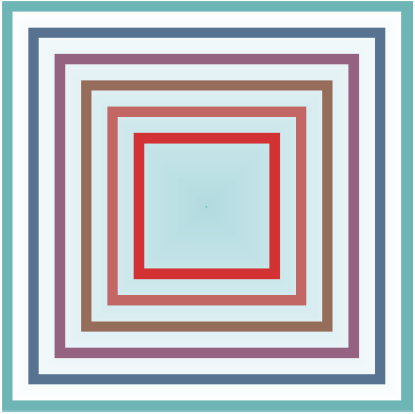
\includegraphics[scale=0.06]{PSCC_logo.png}\\\small{PSCC 2026} \end{minipage} \hfill \small{Limassol, Cyprus --- June 8 -- June 12, 2026}}%
}

\begin{document}

\onecolumn

\title{Stochastic Harmonic Hosting Capacity  \\ under Network Impedance Uncertainty}

\author{
\IEEEauthorblockN{Amauri G. Martins Britto\orcidlink{0000-0002-2691-9061}, Tom Van Acker\orcidlink{0000-0001-6283-1457}, and Hakan Ergun\orcidlink{0000-0001-5171-1986}}
\IEEEauthorblockA{\textit{Department of Electrical Engineering} \\
\textit{KU Leuven} / \textit{EnergyVille - Etch} \\
Leuven / Genk, Belgium\\ }}

\maketitle

{\it Index terms} -- Harmonic distortion, impedance uncertainty, hosting capacity, stochastic optimization.\thanksto{\noindent This work is supported by the Energy Transition Fund by FOD Economy, Belgium, project HARMONIC. The General Board on Energy of the FOD Economy is not liable for any use of the presented work and subsequent results.}

\section{Motivation}
The decarbonization of the global economy requires the electrification of the entire energy system. In the coming decades, the power grid will be dominated by converter-based resources to integrate photovoltaic and wind generation, as well as new types of electrical demand. Traditionally, the hosting capacity of converter-based resources within a given power system has been approached from the perspective of congestion or voltage management; however, recently harmonic distortion has become an increasingly relevant metric~\cite{sun_distribution_2022}.

\section{Novel Contributions}
In the literature, the harmonic hosting capacity problem has mainly been analyzed from a deterministic point of view. Some examples of stochastic approaches have been limited to the amount of harmonic currents injected by devices, or the loading conditions of the network \cite{bozicek_harmonic_2018}. However, an important source of uncertainty that affects the harmonic hosting capacity is the impedance of the network at higher frequencies. This uncertainty is mainly driven by the physical/geometrical properties of passive grid elements and their grounding. This uncertainty affects the grid resonance frequency, which is one of the drivers limiting the harmonic hosting capacity \cite{tom_van_acker_impact_2025}. This paper presents a stochastic optimization model to determine the harmonic hosting capacity in power grids, where the impedance uncertainty is quantified using detailed overhead line and cable models \cite{martins-britto_multilayer_2020}. 

\section{The Proposed Approach}

Building on the deterministic mathematical framework presented in~\cite{tom_van_acker_exact_nodate}, the harmonic impedance uncertainty of overhead lines and underground cables is introduced as robust bounds to the optimization problem. \textit{The result of the presented method is a harmonic current budget for all power system users distributed using a fairness principle that respects the technical limits, e.g., individual or total harmonic distortion limits, for any realization of the harmonic impedance uncertainty.}
To reliably determine the harmonic impedance uncertainty, an open-source toolbox has been developed which focuses on calculating line and cable impedances and admittances in the frequency-domain, accounting for skin effect, insulation properties, and earth-return impedances with frequency-dependent soil models \cite{amauri_g_martins_britto_linecablemodelsjl_nodate}. Using the toolbox, robust bounds on the harmonic impedance are derived, which are embedded in the harmonic hosting capacity optimization problem. 

\section{Numerical Experiments and Validation}
The paper presents two numerical illustrations of the stochastic harmonic hosting capacity problem. First, a five-bus section of a real-world industrial power system is used to validate the methodology. Next, a large-scale transmission system is considered to statistically analyze the effect of harmonic impedance uncertainty in high-voltage grids.

\bibliographystyle{IEEEtran}
\bibliography{journals/dhhc/harmonic_references}

\end{document}